\documentclass[12pt, a4paper]{article}

% --- Packages ---
\usepackage[utf8]{inputenc}
\usepackage[margin=1in]{geometry} % Standard margins
\usepackage{graphicx} % To include images/schematics
\usepackage{amsmath} % For mathematical formulas
\usepackage{titlesec} % For custom section styling
\usepackage{booktabs} % For professional-looking tables
\usepackage{fancyhdr} % For headers and footers
\usepackage{tikz}
\usetikzlibrary{shapes,arrows.meta,positioning,calc}
\usepackage{pgfplots}

% --- Header/Footer Setup ---
\pagestyle{fancy}
\fancyhf{}
\rhead{Spring 2026}
\chead{Basic Electronics Project}
\lhead{
\includegraphics[width=1cm]{HU Logo.png}}
\cfoot{\thepage}
\setlength{\headheight}{32.80098pt}
\addtolength{\topmargin}{-20.80098pt}
\pgfplotsset{compat=1.18}
\begin{document}
    % --- Title Page ---
    \begin{titlepage}
        \centering
        
\includegraphics[width=0.6\textwidth]{HU Logo.png}
        \\
        \vspace*{1cm}
        \Large \textbf{EE-211L Basic Electronics} \\
        \Large Spring 2026 \\
        \huge \textbf{Project Proposal: Cascaded Amplifier} \\
        \vfill
        \Large \textbf{Team Members:} \\
        \Large Tehniyat Ayub (ta10600) \& Mohammad Yousuf Lali (ml10014) \\
        \vfill
        \Large \textbf{Instructor:} \\
        \Large Miss Hira Mustafa \\
        \vspace{0.8cm}
    \end{titlepage}

    % --- Main Content ---
    \section{Objective}
    Design and implement a cascaded amplifier for a 10mV input signal using BJTs (2N3904), ensuring high voltage gain, impedance matching and stable signal amplification.

    \section{Introduction}
    Common Emitter (CE) and Common Collector (CC) amplifiers are essential components in electronic circuits, used to enhance weak signals for further processing. 
    A single-stage amplifier typically provides a voltage gain of up to about 20 before distortion or clipping occurs.
    To overcome these limitations, cascaded amplifiers are used, where multiple amplifier stages are connected in sequence to improve overall performance.
    \\
    \\In this project, we will design a five-stage cascaded amplifier using the following \\configuration:
    \begin{center}
        CE - CC - CE - CC - CE 
    \end{center}
\begin{itemize}
\item CE Stages – Used for voltage gain, provides high amplification but has high output impedance.
\item CC Stages – Used for impedance matching, acts as a buffer, ensuring efficient signal transfer by offering high input and low output impedance.
\end{itemize}
This combination offers an amplifier design that ensures:
\begin{itemize}
\item High overall voltage gain through the CE stages.
\item Proper impedance matching in the CC stage for efficient signal transfer.
\item Improved stability and reduced loading effects, preventing signal clipping.
\end{itemize}
We will ensure that the designed amplifier meets the required performance criteria for amplification by carefully selecting component values and biasing techniques.

    \section{Block Diagram}
    \begin{tikzpicture}[
    node distance=2cm and 0.6cm, % distance between nodes
    box/.style={rectangle, draw, text width=2.5cm, align=center, minimum width=3cm, minimum height=2cm, font=\large},
    connector/.style={->, thick, >=Stealth}
]

    % Nodes
    \node[box] (A) {Input Signal};
    \node[box, right=of A] (B1) {$1^{\text{st} }$ CE Amplifier};
    \node[box, right=of B1] (B2) {$1^{\text{st} }$ CC Amplifier};
    \node[box, right=of B2] (B3) {$2^{\text{nd} }$ CE Amplifier};
    \node[box, right=of B3] (B4) {$2^{\text{nd} }$ CC Amplifier};
    \node[box, below=of B4] (B5) {$3^{\text{rd} }$ CE Amplifier};
    \node[box, left=of B5] (B6) {Load};
    \node[box, left=of B6] (B7) {Output Signal};

    % Connections
    \draw [connector] (A) -- (B1);
    \draw [connector] (B1) -- (B2);
    \draw [connector] (B2) -- (B3);
    \draw [connector] (B3) -- (B4);
    \draw [connector] (B4) -- (B5);
    \draw [connector] (B5) -- (B6);
    \draw [connector] (B6) -- (B7);
    \end{tikzpicture}

    \section{Proposed Schematic}
    \begin{center}
        % Insert your circuit schematic here
        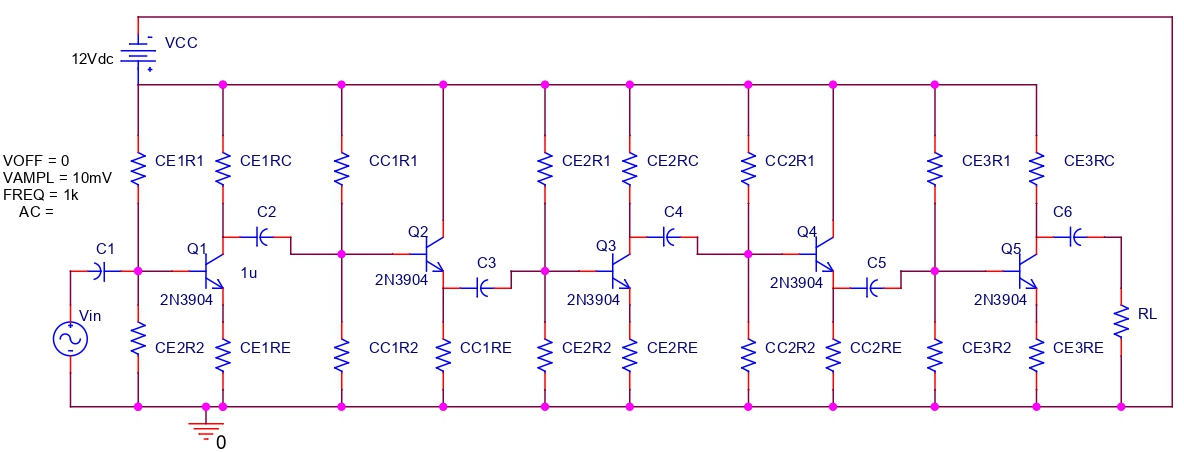
\includegraphics[width = 16cm]{Schematic.png}
    \end{center}
    \section{List of Components}
    \begin{itemize}
        \item \textbf{Resistors}
        \item \textbf{Capacitors} 
        \item \textbf{2N3904 BJTs}
        \item \textbf{Function Generator}
        \item \textbf {DC Power Supply}
    \end{itemize}
    \section{Expected Outcome}
    With this five-stage cascaded amplifier we are aiming
    that a 10 mV input signal will be amplified to approximately 10 V, corresponding to an overall voltage gain of about 1000
    and proper impedance matching for minimal loss 
    and no signal clipping.
    \section{Task Division}
    \begin{table}[h]
        \centering
        \begin{tabular}{|@{}c|c|c@{ }|}
            \hline
            \textbf{ S.No} & \textbf{Task}      & \textbf{Member } \\
            \hline
            1             & Calculations & Tehniyat             \\
            \hline
            2             & Report Generation  & Yousuf            \\
            \hline
            3             & Simulation      & Both             \\
            \hline
            4             & Physical Circuit      & Both              \\
            \hline
            5             & Analysis and Debugging      & Both              \\
            \hline
        \end{tabular}
        \caption{Task Division}
        \label{Table 1}
    \end{table}
\end{document}